\documentclass[10pt,a4paper]{article}
\usepackage[utf8]{inputenc}
\usepackage[T1]{fontenc}
\usepackage[romanian]{babel}
\usepackage[margin=1.7cm]{geometry}
\usepackage{amsmath,amssymb,mathtools}
\usepackage{enumitem}
\usepackage{titlesec}
\usepackage{parskip}
\usepackage{tikz}
\usetikzlibrary{calc}
\usepackage{pgfplots}
\pgfplotsset{compat=1.18}
\usepackage[most]{tcolorbox}

\newtcolorbox{res}{colback=red!6,colframe=red!65!black,boxrule=0.6pt,arc=1.5pt,
  left=4pt,right=4pt,top=2pt,bottom=2pt,breakable}

\setlist{nosep, topsep=2pt, itemsep=2pt, leftmargin=1.3em}
\titlespacing*{\section}{0pt}{6pt}{2pt}
\titlespacing*{\subsection}{0pt}{4pt}{1pt}
\renewcommand{\baselinestretch}{0.96}
\setlength{\parindent}{0pt}
\pagestyle{empty}

\begin{document}
\begin{center}
{\large\bfseries Rezolvare --- Model de antrenament TS2}
\end{center}
\vspace{-0.2cm}

\section*{1. $G_0(s)=\dfrac{2s+3}{s^2+7s+10}=\dfrac{2s+3}{(s+2)(s+5)}$}

\subsection*{a) Model la stare}
$a_1=7,\ a_0=10,\ b_1=2,\ b_0=3$
\begin{res}
$$A=\begin{pmatrix}0&1\\-10&-7\end{pmatrix},\ B=\begin{pmatrix}0\\1\end{pmatrix},\ C=\begin{pmatrix}3&2\end{pmatrix},\ D=0$$
\end{res}

\subsection*{b) Schema bloc}
\begin{center}
\begin{tikzpicture}[scale=0.85, every node/.style={font=\scriptsize}]
\node (u) at (0,0) {$u$};
\node[draw,circle,minimum size=0.5cm] (s1) at (1.1,0) {$\Sigma$};
\draw[->] (u)--(s1);
\node[draw,minimum width=1cm,minimum height=0.6cm] (i1) at (2.7,0) {$\int$};
\draw[->] (s1)--(i1);
\coordinate (a) at (4.3,0);
\draw[->] (i1) -- (a) node[above,pos=0.4]{$x_2$};
\filldraw (a) circle (1pt);
\node[draw,minimum width=1cm,minimum height=0.6cm] (i2) at (5.9,0) {$\int$};
\draw[->] (a) -- (i2);
\coordinate (b) at (7.5,0);
\draw[->] (i2) -- (b) node[above,pos=0.4]{$x_1$};
\filldraw (b) circle (1pt);
\node[draw,circle,minimum size=0.5cm] (sy) at (9.3,0) {$\Sigma$};
\draw[->] (b) -- (sy) node[midway,above]{\tiny $3$};
\draw[->] (a) -- ++(0,1.4) -| (sy.north);
\node[above] at (6.8,1.4){\tiny $2$};
\draw[->] (sy) -- (10.4,0) node[right]{$y$};
\draw[->] (b) -- ++(0,-1.6) -| (s1.south);
\node[below] at (4.3,-1.6){\tiny $-10$};
\draw[->] (a) -- ++(0,-0.9) -| ($(s1.south)+(0.25,0)$);
\node[below] at (2.9,-0.9){\tiny $-7$};
\end{tikzpicture}
\end{center}

\subsection*{c) Răspuns la treaptă unitară}
$$Y(s)=\frac{G_0(s)}{s}=\frac{2s+3}{s(s+2)(s+5)}=\frac{A}{s}+\frac{B}{s+2}+\frac{C}{s+5}$$
$$A=\frac{3}{2\cdot5}=\frac{3}{10}\qquad B=\frac{-4+3}{(-2)(3)}=\frac16\qquad C=\frac{-10+3}{(-5)(-3)}=-\frac{7}{15}$$
\begin{res}
$$y(t)=\frac{3}{10}+\frac16e^{-2t}-\frac7{15}e^{-5t}$$
\end{res}

\subsection*{d) Controlabilitate}
$$AB=\begin{pmatrix}1\\-7\end{pmatrix},\quad P=(B\ AB)=\begin{pmatrix}0&1\\1&-7\end{pmatrix},\quad \det P=-1\ne0$$
\begin{res}
Controlabil.
\end{res}

\section*{2. $G(s)=8\dfrac{0.25s+1}{s}$}

\subsection*{a) Bode}
$$k=8,\ T=0.25\Rightarrow \omega_f=\frac1T=4,\quad k_{dB}=20\lg8=18.06\text{ dB}$$
\begin{res}
$$|G(j\omega)|=\frac{8\sqrt{1+(0.25\omega)^2}}{\omega}\qquad |G(j\omega)|_{dB}=18.06+20\lg\sqrt{1+(0.25\omega)^2}-20\lg\omega$$
$$\varphi(\omega)=\arctan(0.25\omega)-90^\circ$$
\end{res}
Asimptotic: pantă $-20$ dB/dec pt $\omega<4$ (trece prin $(\omega{=}1,\,18.06\text{ dB})$), devine $0$ dB/dec pt $\omega>4$.
Valoare asimptotică la $\omega_f{=}4$: $18.06-20\lg4=6.02$ dB (exact: $9.03$ dB, corecție $+3$ dB).
$$\varphi(0)=-90^\circ,\quad \varphi(4)=\arctan(1)-90^\circ=-45^\circ,\quad \varphi(\infty)=0^\circ$$

\begin{center}
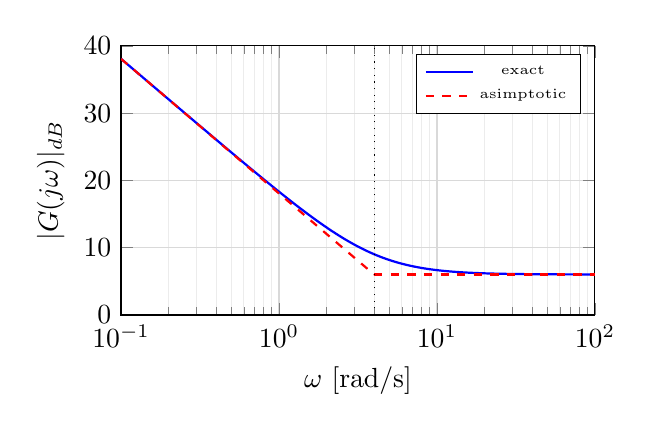
\begin{tikzpicture}
\begin{semilogxaxis}[
  width=7.6cm,height=5cm,
  xlabel={$\omega$ [rad/s]}, ylabel={$|G(j\omega)|_{dB}$},
  xmin=0.1,xmax=100,ymin=0,ymax=40,
  grid=both, minor grid style={gray!15}, major grid style={gray!30},
  legend style={font=\tiny}, legend pos=north east,
]
\addplot[blue,thick,domain=0.1:100,samples=200]
  {20*ln(8)/ln(10)+20*ln(sqrt(1+(0.25*x)^2))/ln(10)-20*ln(x)/ln(10)};
\addlegendentry{exact}
\addplot[red,dashed,thick,domain=0.1:4,samples=50] {20*ln(8)/ln(10)-20*ln(x)/ln(10)};
\addplot[red,dashed,thick,domain=4:100,samples=50] {20*ln(8)/ln(10)-20*ln(4)/ln(10)};
\addlegendentry{asimptotic}
\addplot[black,dotted] coordinates {(4,0)(4,40)};
\end{semilogxaxis}
\end{tikzpicture}
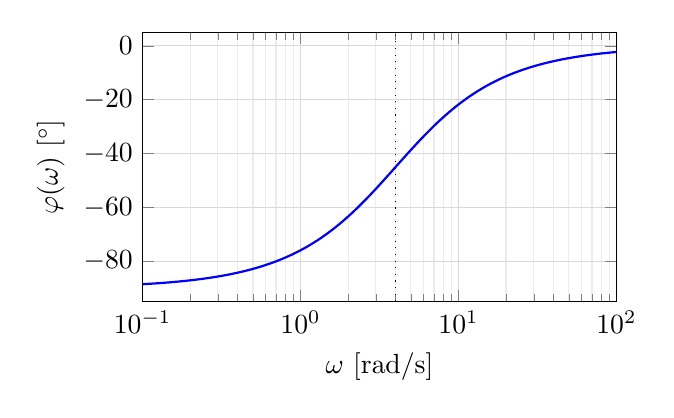
\begin{tikzpicture}
\begin{semilogxaxis}[
  width=7.6cm,height=5cm,
  xlabel={$\omega$ [rad/s]}, ylabel={$\varphi(\omega)$ [$^\circ$]},
  xmin=0.1,xmax=100,ymin=-95,ymax=5,
  grid=both, minor grid style={gray!15}, major grid style={gray!30},
]
\addplot[blue,thick,domain=0.1:100,samples=200] {atan(0.25*x)-90};
\addplot[black,dotted] coordinates {(4,-95)(4,5)};
\end{semilogxaxis}
\end{tikzpicture}
\end{center}

\subsection*{b) Erori staționare}
$$K_p=\lim_{s\to0}G(s)=\infty,\qquad K_v=\lim_{s\to0}sG(s)=8,\qquad K_a=\lim_{s\to0}s^2G(s)=0$$
\begin{res}
$$e_{ss}(\text{treaptă})=\frac1{1+K_p}=0\qquad e_{ss}(\text{rampă})=\frac1{K_v}=\frac18=0.125\qquad e_{ss}(\text{parabolă})=\frac1{K_a}=\infty$$
\end{res}

\section*{3. $G(s)=\dfrac{k}{s(s+4)},\ H(s)=\dfrac1{s+2}$}

$$L(j\omega)=\frac{k}{-6\omega^2+j\omega(8-\omega^2)}$$

\subsection*{a) Curba polară \& domeniu de stabilitate}
$$\mathrm{Im}\{L(j\omega)\}=0\Rightarrow \omega(8-\omega^2)=0\Rightarrow \omega_\pi=2\sqrt2\approx2.828$$
$$\mathrm{Re}\{L(j\omega_\pi)\}=\frac{k}{-6\cdot8}=-\frac{k}{48}$$
\begin{res}
$$-\frac{k}{48}>-1\ \Rightarrow\ k<48 \qquad\Rightarrow\qquad 0<k<48$$
\end{res}
$$\mathrm{Re}(\omega)=\frac{-6k\omega^2}{36\omega^4+\omega^2(8-\omega^2)^2}\qquad \mathrm{Im}(\omega)=\frac{-k\omega(8-\omega^2)}{36\omega^4+\omega^2(8-\omega^2)^2}$$
Puncte de control (ex. $k=20$):
\begin{center}
\begin{tabular}{@{}lll@{}}
$\omega\to0^+$: & $\mathrm{Re}\to0$, & $\mathrm{Im}\to-\infty$ ($\varphi\to-90^\circ$)\\
$\omega=1$: & $\mathrm{Re}=-1.412$, & $\mathrm{Im}=-1.647$\\
$\omega=\omega_\pi=2.828$: & $\mathrm{Re}=-0.417$, & $\mathrm{Im}=0$\\
$\omega=5$: & $\mathrm{Re}=-0.101$, & $\mathrm{Im}=0.057$\\
$\omega\to\infty$: & $\mathrm{Re}\to0$, & $\mathrm{Im}\to0^+$ ($\varphi\to-270^\circ$)\\
\end{tabular}
\end{center}

\begin{center}
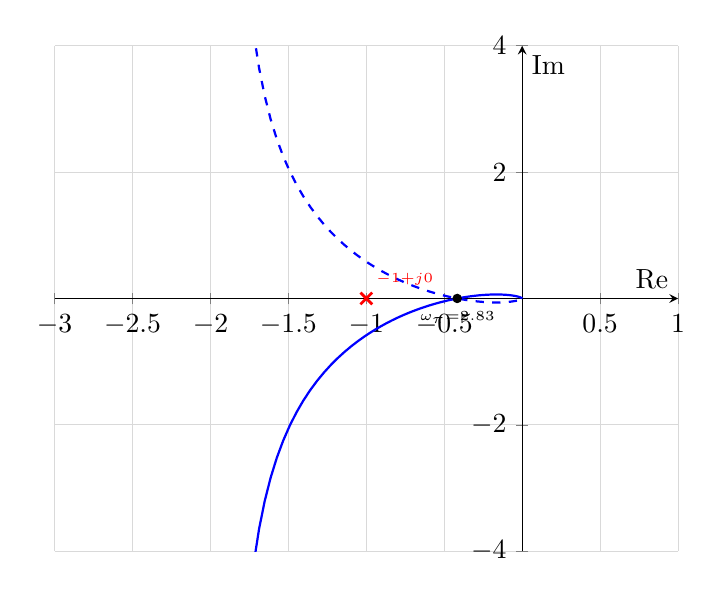
\begin{tikzpicture}
\begin{axis}[
  width=9.5cm,height=8cm,
  xlabel={$\mathrm{Re}$}, ylabel={$\mathrm{Im}$},
  xmin=-3,xmax=1,ymin=-4,ymax=4,
  axis lines=middle,
  grid=both, minor grid style={gray!15}, major grid style={gray!30},
]
\addplot[blue,thick,samples=500,domain=0.05:30,variable=\w]
  ({-6*20*\w^2/(36*\w^4+\w^2*(8-\w^2)^2)},{-20*\w*(8-\w^2)/(36*\w^4+\w^2*(8-\w^2)^2)});
\addplot[blue,thick,dashed,samples=500,domain=0.05:30,variable=\w]
  ({-6*20*\w^2/(36*\w^4+\w^2*(8-\w^2)^2)},{20*\w*(8-\w^2)/(36*\w^4+\w^2*(8-\w^2)^2)});
\addplot[only marks,mark=x,red,mark size=3pt,line width=1pt] coordinates {(-1,0)};
\node[red,anchor=south west] at (axis cs:-1,0.05) {\tiny $-1{+}j0$};
\addplot[only marks,mark=*,black,mark size=1.5pt] coordinates {(-0.417,0)};
\node[anchor=north] at (axis cs:-0.417,-0.05) {\tiny $\omega_\pi{=}2.83$};
\end{axis}
\end{tikzpicture}
\end{center}

\subsection*{b) Marginea de fază (ex. $k=20$)}
$$|L(j\omega_t)|=1\Rightarrow 36\omega_t^4+\omega_t^2(8-\omega_t^2)^2=k^2=400$$
$$x=\omega_t^2:\quad x^3+20x^2+64x-400=0\ \Rightarrow\ x\approx3.005\ \Rightarrow\ \omega_t\approx1.733$$
$$\varphi(\omega_t)=-90^\circ-\arctan\frac{\omega_t}{4}-\arctan\frac{\omega_t}{2}=-90^\circ-23.42^\circ-40.94^\circ=-154.36^\circ$$
\begin{res}
$$\gamma=180^\circ+\varphi(\omega_t)=25.64^\circ$$
\end{res}

\section*{4. $G(s)=\dfrac{K(s+4)}{s(s+3)(s^2+2s+5)}$}
Poli: $0,\ -3,\ -1{\pm}2j$ ($n=4$). Zero: $-4$ ($m=1$).

\subsection*{Asimptote}
\begin{res}
$$n-m=3,\quad \theta_k=\frac{180^\circ(2k+1)}{3}=60^\circ,\,180^\circ,\,300^\circ$$
$$\sigma_a=\frac{(0-3-1-1)-(-4)}{3}=\frac{-1}{3}\approx-0.333$$
\end{res}

\subsection*{Unghi de plecare din $-1+2j$}
Vectori de la ceilalți poli: din $0\to(-1{+}2j)$: $116.57^\circ$; din $-3\to(-1{+}2j)$: $45^\circ$; din $-1{-}2j\to(-1{+}2j)$: $90^\circ$ (sumă $251.57^\circ$).
Vector de la zero: din $-4\to(-1{+}2j)$: $33.69^\circ$.
\begin{res}
$$\varphi_p=180^\circ-251.57^\circ+33.69^\circ=-37.88^\circ \qquad(\text{din }-1{-}2j:\ +37.88^\circ,\text{ prin simetrie})$$
\end{res}

\subsection*{Puncte de rupere}
$$K(s)=-\frac{s(s+3)(s^2+2s+5)}{s+4}=-\frac{s^4+5s^3+11s^2+15s}{s+4}$$
$$\frac{dK}{ds}=-\frac{3s^4+26s^3+71s^2+88s+60}{(s+4)^2}=0\ \Rightarrow\ 3s^4+26s^3+71s^2+88s+60=0$$
\begin{res}
$s\approx-2.32$ (rupere, pe segmentul $(-3,0)$) \quad și\quad $s\approx-4.85$ (intrare, pe segmentul $(-\infty,-4)$)
\end{res}
Segmente reale ale locului (regulă impar): $(-3,0)$ și $(-\infty,-4)$.

\subsection*{Intersecția cu axa imaginară}
Ecuație caracteristică: $s^4+5s^3+11s^2+(15+K)s+4K=0$, cu $s=j\omega$:
$$\text{Re}:\ \omega^4-11\omega^2+4K=0\qquad \text{Im}:\ \omega(15+K-5\omega^2)=0\Rightarrow\omega^2=\frac{15+K}{5}$$
$$K^2+75K-600=0\ \Rightarrow\ K=\frac{-75+\sqrt{8025}}{2}\approx7.29$$
\begin{res}
$$K\approx7.29\qquad \omega^2=\frac{15+7.29}{5}\approx4.458\ \Rightarrow\ \omega\approx\pm2.11$$
\end{res}

\begin{center}
\begin{tikzpicture}
\begin{axis}[
  width=11cm,height=9.5cm,
  xlabel={$\mathrm{Re}$}, ylabel={$\mathrm{Im}$},
  xmin=-11,xmax=6,ymin=-9.5,ymax=9.5,
  axis lines=middle,
  grid=both, minor grid style={gray!15}, major grid style={gray!30},
]
\addplot[blue,thick] table {rlocus_data/branch0.dat};
\addplot[blue,thick] table {rlocus_data/branch1.dat};
\addplot[blue,thick] table {rlocus_data/branch2.dat};
\addplot[blue,thick] table {rlocus_data/branch3.dat};
\addplot[gray,dashed] coordinates {(-0.333,0)(3.667,6.928)};
\addplot[gray,dashed] coordinates {(-0.333,0)(-10.333,0)};
\addplot[gray,dashed] coordinates {(-0.333,0)(3.667,-6.928)};
\addplot[only marks,mark=x,black,mark size=3pt,line width=1.2pt] coordinates {(0,0)(-3,0)(-1,2)(-1,-2)};
\addplot[only marks,mark=o,black,mark size=3pt,line width=1.2pt] coordinates {(-4,0)};
\addplot[only marks,mark=*,red,mark size=1.6pt] coordinates {(-2.33,0)(-4.85,0)};
\addplot[only marks,mark=*,red,mark size=1.6pt] coordinates {(0,2.11)(0,-2.11)};
\node[anchor=south west] at (axis cs:-2.33,0.15) {\tiny rupere};
\node[anchor=north west] at (axis cs:-4.85,-0.15) {\tiny intrare};
\node[anchor=west] at (axis cs:0.2,2.11) {\tiny $K{\approx}7.29$};
\end{axis}
\end{tikzpicture}
\end{center}

\section*{5. $G(s)=\dfrac{16}{s^2+8s+16}$, $u(t)=3\sin3t$}
$$G(j3)=\frac{16}{(16-9)+8\cdot3j}=\frac{16}{7+24j},\qquad |7+24j|=\sqrt{49+576}=25$$
$$|G(j3)|=\frac{16}{25}=0.64\qquad \varphi=-\arctan\frac{24}{7}=-73.74^\circ$$
\begin{res}
$$y(t)=3\cdot0.64\,\sin(3t-73.74^\circ)=1.92\,\sin(3t-73.74^\circ)$$
\end{res}

\begin{center}
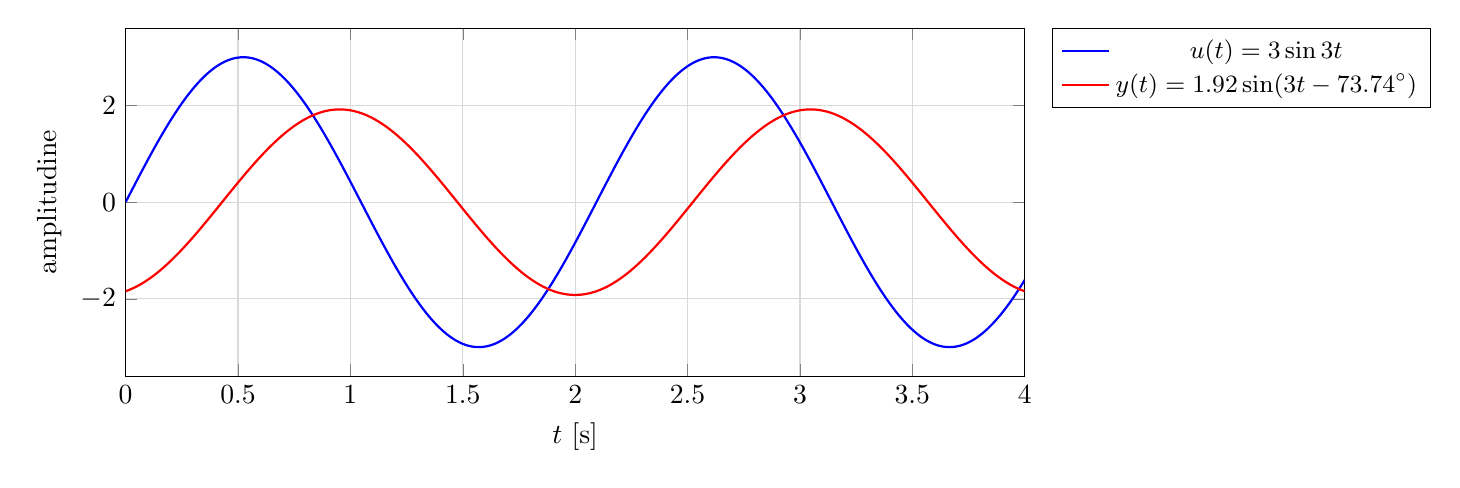
\begin{tikzpicture}
\begin{axis}[
  width=13cm,height=6cm,
  xlabel={$t$ [s]}, ylabel={amplitudine},
  xmin=0,xmax=4,
  grid=both, minor grid style={gray!15}, major grid style={gray!30},
  legend style={font=\small}, legend pos=outer north east,
]
\addplot[blue,thick,domain=0:4,samples=300] {3*sin(deg(3*x))};
\addlegendentry{$u(t)=3\sin3t$}
\addplot[red,thick,domain=0:4,samples=300] {1.92*sin(deg(3*x)-73.74)};
\addlegendentry{$y(t)=1.92\sin(3t-73.74^\circ)$}
\end{axis}
\end{tikzpicture}
\end{center}

\end{document}
